\documentclass[12pt]{article}
\usepackage{amsmath} % For basic math symbols and environments
\usepackage{tikz} % For drawing shapes
\usepackage{enumitem} % For customizing lists
\usepackage[margin=1in]{geometry} % For setting page margins
\usepackage{float} % For better control of figure placement
\usetikzlibrary{shapes.geometric, arrows.meta, positioning}
\usepackage{enumitem} % For customising lists
\usepackage{siunitx} % For units

\title{Proportion Extension Problems}
\date{}

\begin{document}


\maketitle

\section*{Direct Proportion Past}

\begin{enumerate}
    \item A bag of 5 apples costs £1.20. What is the cost of 40\% more apples? How many apples is that?
    \vspace{0.6cm}


    \item If 10\% of a number is 15, what is 40\% of the number?
    \vspace{0.6cm}

    \item A shop offers a 15\% discount for buying 3 of the same item. If one book normally costs £8, how much would 3 books cost with the discount?
    \vspace{0.6cm}

    \item The cost of fuel is directly proportional to the number of litres purchased. If 40 litres cost £68.00, and the price then increases by 5\%, what will 25 litres cost at the new price?
    \vspace{0.6cm}

    \item A coffee shop's revenue is directly proportional to the number of customers. On Monday, they had 120 customers and made £420. On Tuesday, they increased their prices by 8\%. How many customers did they have on Tuesday if their revenue was £453.60?
\end{enumerate}

\vspace{1.2cm}

\newpage{}

\section*{Direct Proportion Future}

\textbf{Instructions:} Solve the following problems involving the perimeter and area of 2D shapes. The shapes are similar unless stated otherwise.

\begin{enumerate}[resume]
    \item The perimeter of a square is directly proportional to the length of its side. If a square with a side of 4 cm has a perimeter of 16 cm, what is the perimeter of a square with a side of 11 cm?
    \vspace{1.2cm}

    \item The length and width of a rectangle are in a direct proportion. A rectangle has a length of 5 cm and a perimeter of 18 cm. What is the perimeter of a rectangle with a length of 15 cm?\\

    \begin{center}
    \begin{tikzpicture}[scale=0.7, baseline=(current bounding box.center)]
        \draw (0,0) rectangle (5, 4);
        \node[above] at (2.5, 4) {5 cm};
        \node[right] at (5, 2) {? cm};
    \end{tikzpicture}
    \end{center}
    
    \vspace{1.2cm}

    \item The area of a square is directly proportional to the square of its side length. If a square with a side of 3 cm has an area of 9 cm$^2$, what is the area of a square with a side of 7 cm?
    \vspace{1.2cm}

    \item Two similar triangles are shown below. The perimeter of the smaller triangle is 21 cm. The side lengths of the larger triangle are 2.5 times those of the smaller one. What is the perimeter of the larger triangle?\\

    \begin{center}
        
    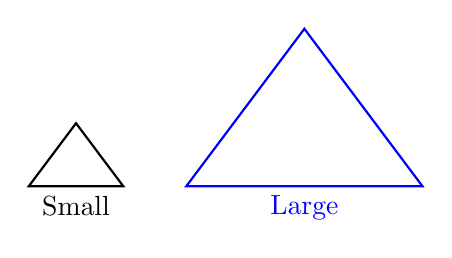
\begin{tikzpicture}[scale=0.4, baseline=(current bounding box.center)]
        % Small Triangle
        \draw[thick] (0,0) -- (3,0) -- (1.5,2) -- cycle;
        \node[below] at (1.5, 0) {Small};
        % Large Triangle
        \draw[thick, blue] (5,0) -- (12.5,0) -- (8.75,5) -- cycle;
        \node[below, blue] at (8.75, 0) {Large};
    \end{tikzpicture}
    \end{center}
    
    \vspace{1.2cm}

    \item A rectangular garden is 10 m long and 6 m wide. A new, similarly shaped garden is to be built. The area of the new garden needs to be 50\% larger than the original.
    \begin{enumerate}[label=(\alph*)]
        \item What is the area of the new garden?
        \item What is the perimeter of the new garden?
    \end{enumerate}
    \begin{tikzpicture}[baseline=(current bounding box.center)]
        \draw (0,0) rectangle (5, 3);
        \node[above] at (2.5, 3) {10 m};
        \node[right] at (5, 1.5) {6 m};
        \node at (2.5, -0.5) {Original Garden};
    \end{tikzpicture}
    \vspace{1.2cm}
\end{enumerate}


\section*{Rates of Change Past}

\begin{enumerate}[resume]

    \item A plant was \SI{20}{\centi\meter} tall. Over the next week, it grew by \textbf{5\%}. At what speed did it grow, in cm per day?
\vspace{0.6cm}
    \item A bathtub fills at a rate of \SI{8}{\litre\per\minute}. The plug is slightly loose, and water drains out at a rate that is 2\% of the fill rate. If the tub starts empty, how much water is in it after 10 minutes?
\vspace{0.6cm}
    \item A car's value was \pounds 15,000. It depreciates (loses value) at a rate of 12\% per year. A motorbike's value was \pounds 8,000 and it depreciates at 8\% per year. After 3 years, which vehicle is worth more? Justify your answer with calculations.
\vspace{0.6cm}
    \item A social media post is shared rapidly. On the first day, it gets 200 shares. The number of shares increases by 15\% each day after that.
    \begin{enumerate}
        \item How many shares does it get on the third day?
        \item What is the total number of shares at the end of the third day?
    \end{enumerate}
\vspace{0.6cm}
    \item A factory's energy costs are \pounds 10,000 per month. The manager invests in new equipment which is 20\% more efficient. However, due to increased production, the factory now runs for 15\% more hours each month, up from 200 hours. Calculate the new energy cost per hour, and per month, assuming cost is directly proportional to running hours.

\end{enumerate}

\section*{Rates of Change Future}

\begin{enumerate}[resume]

    \item A square has a side length that is increasing at a rate of \SI{2}{\centi\meter\per\second}. What is the rate of change of its perimeter when the side length is \SI{5}{\centi\meter}?, what about when the side length is \SI{10}{\centi\meter}? Does the rate depend on the side length?
\vspace{0.6cm}
    \item A rectangular car park is \SI{60}{\metre} long and \SI{40}{\metre} wide. It is to be resurfaced. The cost of resurfacing is \pounds 15 per square metre. Calculate the total cost.
\vspace{0.6cm}
    \item A circular oil spill is spreading. It starts with a radius of 1m. The radius of the spill is increasing at a constant rate of \SI{0.5}{\metre\per\minute}.
    \begin{enumerate}
        \item Calculate the rate at which the \textbf{circumference} of the spill is increasing when the radius is \SI{4}{\metre}. (Use $C = \pi D$)
        \item Calculate the rate at which the \textbf{circumference} of the spill is increasing when the radius is \SI{8}{\metre}.
        \item Find the area of the spill after 10 minutes.  (Use $A = \pi r^2$)
    \end{enumerate}
\vspace{0.6cm}
    \item A gardener is planting a rectangular flower bed. The length of the bed is increasing at a rate of \SI{1}{\metre\per\hour} and the width is increasing at a rate of \SI{0.5}{\metre\per\hour}. At a specific moment, the length is \SI{6}{\metre} and the width is \SI{4}{\metre}.
    \begin{enumerate}
        \item At what rate is the \textbf{perimeter} increasing at this moment?
        \item How much will the \textbf{area} have increased by 30 minutes later? Do you think it grew at a constant rate?
    \end{enumerate}
\vspace{0.6cm}
    \item A decorative path is being built around a rectangular pond. The pond is \SI{10}{\metre} long and \SI{6}{\metre} wide. The path has a uniform width of $x$ metres all the way around.
    \begin{enumerate}
        \item Show that the area of the path, $A$, is given by the formula $A = 4x^2 + 32x$.
        \item If the path is being paved at a rate of \SI{0.8}{\square\metre\per\minute}, how wide is the path after 20 minutes, assuming it is being paved outwards from the rectangle?
    \end{enumerate}

\end{enumerate}

\end{document}
